%!TEX root = ../dokumentation.tex

\chapter{Theoretische Grundlagen}
\section{Elektromagnetische Wellen}
Als elektromagnetische Welle wird eine Welle beschrieben, die aus elektrischen und magnetischen Feldern besteht. 
\section{Frequenzbereiche in der Funktechnik}
\section{Frequenzbereiche}
Zur Orientierung im Spektrum elektromagnetischer Wellen haben sich international verschiedene Systeme zur Klassifikation sogenannter Frequenzbänder gebildet. Die \ac{ITU} empfiehlt eine Einteilung des Spektrums von 3 kHz bis 300 GHz in acht Frequenzbereiche, auch Frequenzdekaden genannt. \cite[vgl. ITU-R v.431-8]{itu-431:2015}

\begin{figure}[ht]
	\centering
	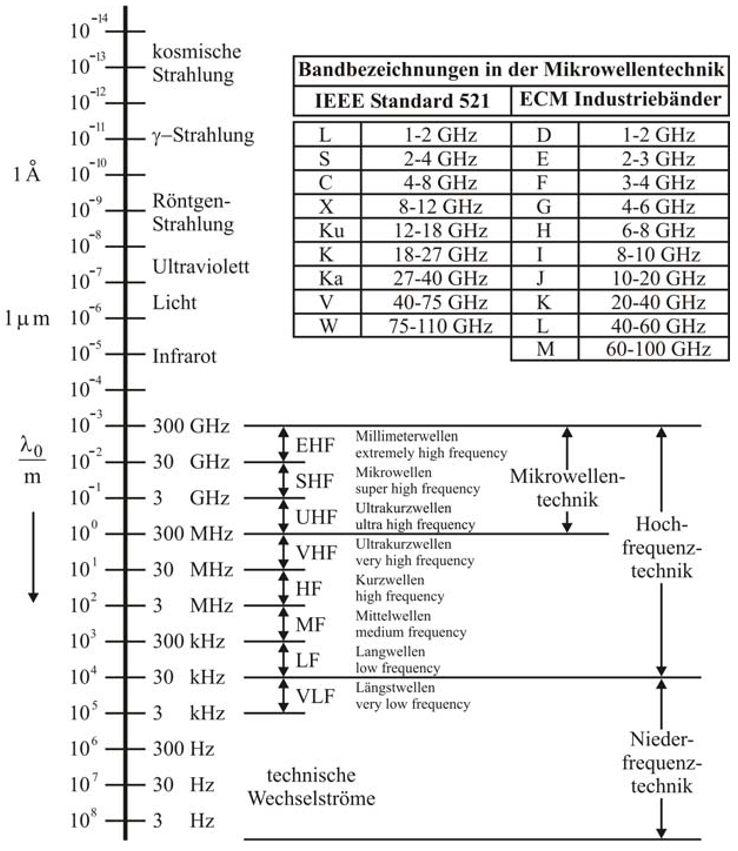
\includegraphics[width=0.75\textwidth]{frequenzbereich.png}
	\caption[Spektrum elektromagnetischer Wellen und gebräuchliche Bandbezeichnungen]{Spektrum elektromagnetischer Wellen und gebräuchliche Bandbezeichnungen. Quelle: \cite[Kark, S. 1]{Kark:2017}} 
	\label{frequenzbereiche}
\end{figure}


\subsection{Rechtliche Grundlagen} %TODO
In Deutschland gilt rechtlich zudem die Aufteilung des Frequenzbereiches von 9 kHz bis 3000 GHz, welche von der Bundesnetzagentur im sogenannten Frequenzplan \cite[Bundesnetzagentur, 2016]{bundesnetzagentur-frequenzplan:2016} gemäß § 54 TKG festgehalten wird.
Dort werden die Frequenzbereiche nach Frequenznutzung (Amateurfunk, Seefunk, WLAN, etc.) eingeteilt und entsprechende Nutzungsbestimmungen spezifiziert:

\begin{figure}[ht]
	\centering
	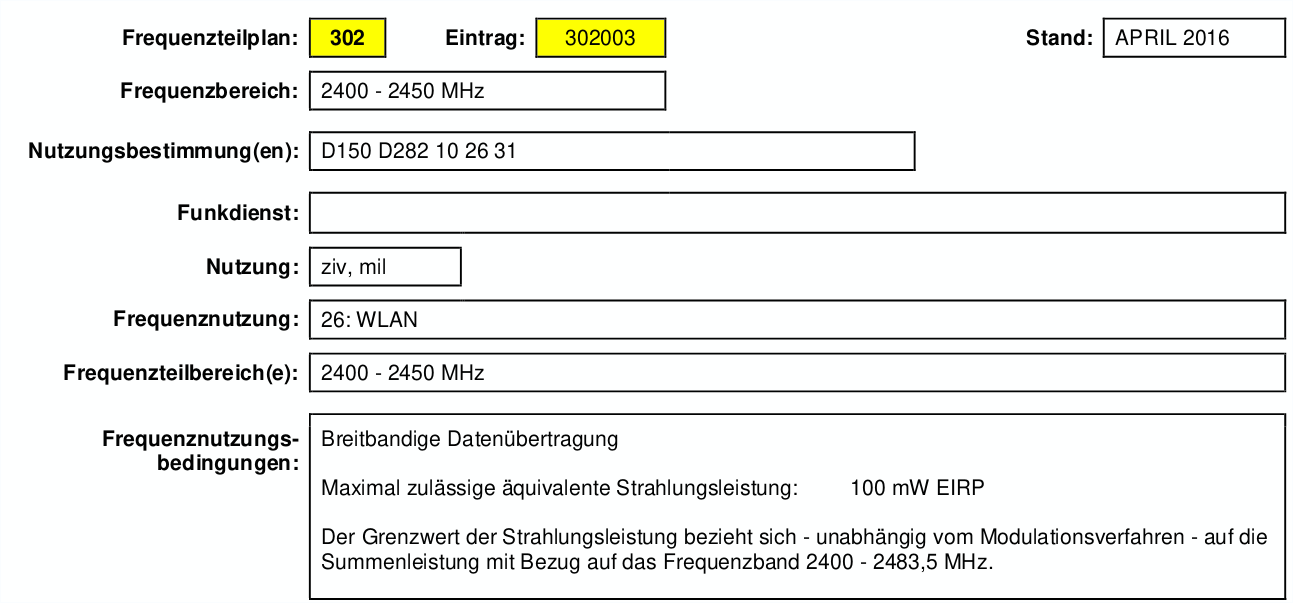
\includegraphics[width=\textwidth]{freqplan-wlan.png}
	\caption[Eintrag: 2,4 GHz WLAN im Frequenzplan]{Eintrag: 2,4 GHz WLAN im Frequenzplan. Quelle: \cite[Bundesnetzagentur, 2016]{bundesnetzagentur-frequenzplan:2016}}
	\label{frequenzplan-wlan}
\end{figure}

\subsection{Dezimeterwelle}
Das Frequenzband von 300 MHz bis 3 GHz, auch \ac{UHF}-Band genannt, ist ein Frequenzbereich in dem die Wellen eine Länge von zehn Dezimeter bis einem Dezimeter besitzen.

\section{Bluetooth}
Bluetooth ist eine Übertragungstechnik für kabellose Kommunikation über kurze Distanzen. Es wird im Frequenzbereich von 2,4 bis 2,4835 GHz betrieben \cite[Bundesamt für Strahlenschutz, S. 1]{bundesamt-strahlungsschutz:2012}. Insgesamt gibt es unter Bluetoothgeräten drei verschiedene Sendeleistungsklassen:
\begin{description}
	\item[Klasse 1: bis 1,0 mW] Reichweite: bis 10m 
	\item [Klasse 2: bis 2,5 mW] Reichweite: 10m und mehr
	\item [Klasse 3: bis 100 mW] Reichweite: 100m und mehr
\end{description}
Die Aufteilung des Frequenzbereiches von 0 kHz bis 3000 GHz wird von der Bundesnetzagentur im sogenannten Frequenzplan \cite[Bundesnetzagentur]{bundesnetzagentur-frequenzplan:2016} gemäß § 54 TKG festgehalten.

\section{Wireless Local Area Network}
Unter dem Begriff Wireless Local Network (WLAN) versteht man ein kabelloses lokales Netzwerk, welches meist an Orten eingesetzt wird, bei der kabelgebundene Datenübertraung zu teuer, umständlich oder umkomfortabel wäre.

\section{Software Defined Radio} 
\enquote{Funkübertragungssysteme, bei denen wesentliche Teile der Verarbeitung mittels Software erfolgen, werden als Software Defined Radio \ac{SDR}-Systeme bezeichnet.} \cite[Heuberger, e. a., S. 1]{Heuberger:2017}


